In the second sprint the \gls{rs} system were designed to consists of three parts: The app, the \gls{rs} server, and the \gls{astep} system.
As the \gls{astep} system have evolved small redesigns to the \gls{rs} system design is necessary.

This section will describe how the communication between the \gls{rs} system and the \gls{astep} system is handled.
And how features from the \gls{astep} API is used to achieve the desired outcomes.

The \gls{astep} API is, as described in Section \ref{ssec:communicationwithastep}, a REST API. 
This means that all API calls are done through HTTP requests\footnote{Overview of all the HTTP-request available in \gls{astep} can be found at \url{http://www.astep.cs.aau.dk/}}.

We will only be using a subset of the features presented to us, those being; Locations, Routes, Users, and some way to allow \gls{rs} to access the data from the \gls{astep} server for its users.
In the API there are two ways of doing this; by creating a group for all the app users or by having an edge from a separate \gls{rs}-user to every \gls{astep}-user that uses the app.

\paragraph{Groups} in the \gls{astep} program exists to allow users to gain access to each others data.
This could be used by making a user for the \gls{rs} system where all users who uses the app is included in.
The problem with this is that all users have now granted access to their local data to anyone how happens to use the same app, regardless of the context. 
This means that a malicious programmer could create a program that plots the locations of all users of the \gls{rs} app.
They would only need a new user registered as using the \gls{rs} app and would there for be included in the group.

\begin{figure}[h]
	\centering
	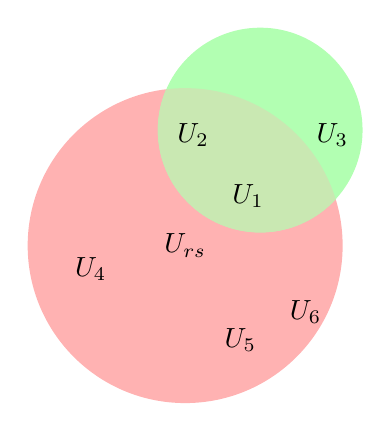
\begin{tikzpicture}
		\path[fill=red!30] (0:0cm) circle (2cm);
		\path[fill=green!30] (57:1.75cm) circle (1.3cm);
	
		\begin{scope}
			\clip(57:1.75cm) circle (1.3cm);
			\path[fill=red!30!green!30] (0:0cm) circle (2cm);
		\end{scope}
		
		\node at (0,	0) 		{$U_{\gls{rs}}$};
		\node at (0.8,	0.63) 	{$U_1$};
		\node at (0.1,	1.4)	{$U_2$};
		\node at (1.87,	1.4) 	{$U_3$};
		\node at (-1.2,	-0.3)	{$U_4$};
		\node at (0.7,	-1.2) 	{$U_5$};
		\node at (1.53, -0.84) 	{$U_6$};
	\end{tikzpicture}
	\label{fig:astepgroup}
	\caption{How the \gls{rs}-system would use groups. In the red group (the red circle) all users in that group can see all data from other users in the same group.}
\end{figure}

\paragraph{Edges} works is a similar way to groups but instead of granting all users access to every other users data, the edges only allow access from one user to another.
Using the same method of establishing communication as with the groups we create a \gls{rs}-user and creates a edge from that user to every user in the \gls{rs} system.
This way it is only when the \gls{rs} system uses its own user it is allowed to access data from the users.

\begin{figure}[h]
	\centering
	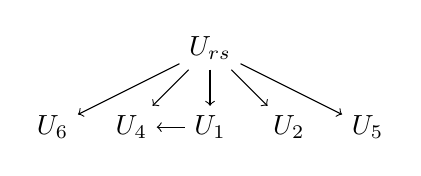
\begin{tikzpicture}
		
		\node (r) {$U_{\gls{rs}}$};
		\node[below of=r] (1) {$U_1$};
		\node[right of=1](2) {$U_2$};
		\node[left of=1] (4) {$U_4$};
		\node[right of=2] (5) {$U_5$};
		\node[left of=4] (6) {$U_6$};
		
		\draw[->] (r) -- (1);
		\draw[->] (r) -- (2);
		\draw[->] (r) -- (4);
		\draw[->] (r) -- (5);
		\draw[->] (r) -- (6);
		
		\draw[->] (1) -- (4);
	\end{tikzpicture}
	\label{fig:astepgroup}
	\caption{How the \gls{rs}-system would work with edges.}
\end{figure}

This means that edges can provide the same benefits without opening the same security flaws.
Therefor the edges is determined to be the superior system.

A  overview of every API calls, as of sprint 3, required by the \gls{rs}-system can be seen on Table \ref{tab:asteprequests}.

\begin{table}[h]
	\centering
	\scriptsize
	\begin{tabular}{l l l}
		Path & Method & Description\\\midrule
		/locations/outdoor/\{username\}/routes & POST & Send a route to the \gls{astep} server\\
		/locations/outdoor/\{username\}/routes/match & GET & Match all new routes\\
		/users & POST & Create a new user\\
		/users/\{username\}/outUsers & POST & Request a new out user\\
		/users/\{username\}/outUsers/\{specifiedUsername\} & PUT & Accept out user\\
		/users/\{username\}/token & GET & Get the current valid token for a user
	\end{tabular}
	\label{tab:asteprequests}
	\caption{}
\end{table}

In sprint 2 it was also decided to created a user through the \gls{rs} server, this have been changed to simplify the implementation.
When a user registers in the app an API call will be issued to the \gls{astep} API directly from the app where before this was done through the \gls{rs} server. 
The username and the additional information such as phone number and full name are still transfered to the \gls{rs} server for storing.